% Báo cáo đồ án Xử lý ảnh — nhóm MedTrack
% Biên dịch: latexmk   (cấu hình trong .latexmkrc: XeLaTeX + biber, kết quả ở build/main.pdf)
% File này giữ thứ tự các mục; nội dung nằm trong sections/, appendix/, refs/ (phân công viết: ../guidelines.md).
\documentclass[11pt,a4paper]{article}

% ---------- Ngôn ngữ, phông chữ ----------
\usepackage{fontspec}
\usepackage[vietnamese]{babel}
% TeX Gyre Termes: tương đương Times, đủ dấu tiếng Việt, có sẵn trong MiKTeX / TeX Live (gọi theo tên file để chạy được trên mọi máy)
\setmainfont{texgyretermes}[Extension=.otf, UprightFont=*-regular, BoldFont=*-bold,
  ItalicFont=*-italic, BoldItalicFont=*-bolditalic]

% ---------- Trang ----------
\usepackage[a4paper,left=3cm,right=2cm,top=2cm,bottom=2cm]{geometry}  % lề theo quy chuẩn văn bản
\usepackage{setspace}\setstretch{1.12}                % giãn dòng cho dễ đọc
% Đoạn văn: không thụt đầu dòng, cách nhau một khoảng trắng
\setlength{\parindent}{0pt}
\setlength{\parskip}{0.5em plus 0.2em minus 0.1em}
\usepackage{titlesec}
\titleformat{\section}{\Large\bfseries}{\thesection}{0.8em}{}
\titleformat{\subsection}{\large\bfseries}{\thesubsection}{0.8em}{}
\titleformat{\subsubsection}{\normalsize\bfseries}{\thesubsubsection}{0.8em}{}
\titlespacing*{\section}{0pt}{2.5ex plus 1ex}{1.2ex}
\titlespacing*{\subsection}{0pt}{2ex plus 0.5ex}{0.8ex}
\titlespacing*{\subsubsection}{0pt}{1.6ex plus 0.5ex}{0.5ex}

% ---------- Hình, bảng, toán ----------
\usepackage{graphicx}\graphicspath{{figure/}{result/}}
\usepackage{booktabs,tabularx,multirow,makecell}
\newcolumntype{L}{>{\raggedright\arraybackslash}X}       % cột co giãn, căn trái (không giãn chữ)
\renewcommand{\arraystretch}{1.2}                     % giãn hàng trong bảng
\setlength{\tabcolsep}{7pt}
\usepackage{caption,subcaption}
\captionsetup{font=small,labelfont=bf,skip=8pt}
\captionsetup[table]{position=top}
\usepackage{float}
\setlength{\intextsep}{1.0em plus 0.3em minus 0.2em}  % khoảng cách quanh bảng, hình
\usepackage{amsmath,amssymb}
\AtBeginDocument{%                                     % khoảng cách quanh công thức
  \setlength{\abovedisplayskip}{1.2em plus 0.3em}\setlength{\belowdisplayskip}{1.2em plus 0.3em}%
  \setlength{\abovedisplayshortskip}{0.8em plus 0.2em}\setlength{\belowdisplayshortskip}{1.2em plus 0.3em}}
\usepackage{siunitx}\sisetup{output-decimal-marker={,},group-separator={.}}
\usepackage{enumitem}
\setlist{leftmargin=2em,itemsep=0.35em,topsep=0.6em,parsep=0pt}  % danh sách thoáng, thụt lề rõ
\usepackage{xcolor}
\usepackage{fancyvrb}                                     % khối mã JSON
\usepackage{tikz}\usetikzlibrary{positioning,arrows.meta,calc}

% ---------- Tài liệu tham khảo (IEEE) ----------
\usepackage{csquotes}
\DeclareQuoteAlias{english}{vietnamese}               % csquotes không có kiểu ngoặc tiếng Việt → dùng “…” kiểu Anh
\usepackage[style=ieee,backend=biber,language=english]{biblatex}   % biblatex chưa hỗ trợ tiếng Việt; nguồn trích đều tiếng Anh
\DeclareLanguageMapping{vietnamese}{english}           % không có vietnamese.lbx → dùng chuỗi tiếng Anh (vol., no., pp.)
\addbibresource{refs/common.bib}
\addbibresource{refs/preprocessing.bib}
\addbibresource{refs/cleaning.bib}
\addbibresource{refs/dl.bib}

\usepackage[hidelinks]{hyperref}
\urlstyle{tt}   % \path{...}: đường dẫn file, tự xuống dòng tại dấu /

% ---------- Lệnh dùng chung ----------
\newcommand{\TODO}[1]{\textcolor{red}{[TODO: #1]}}   % chỗ cần viết; phải hết trước khi nộp
\newcommand{\chuong}[1]{(Chương~#1)}                  % ghi chương học phần: \chuong{3}
\newcommand{\KQ}[1]{\textcolor{blue}{[#1]}}  % SỐ LIỆU CHỜ ĐIỀN: thay cả \KQ{...} bằng số; phải hết trước khi nộp
\newcommand{\khoi}[1]{khối~#1}                       % \khoi{A} → khối A
\newcommand{\Khoi}[1]{Khối~#1}                       % đầu câu

\begin{document}

% ===== khối tiêu đề (không tách trang riêng để tiết kiệm số trang) =====
\begin{center}
  {\small HỌC VIỆN CÔNG NGHỆ BƯU CHÍNH VIỄN THÔNG --- KHOA TRÍ TUỆ NHÂN TẠO}\\[0.4em]
  {\small ĐỒ ÁN MÔN XỬ LÝ ẢNH \quad·\quad Giảng viên: PGS.TS.\ Phạm Văn Cường}\\[0.8em]
  {\Large\bfseries Pipeline tiền xử lý, phân loại và bóc tách cấu trúc\\[0.2em]
   tài liệu y tế từ ảnh chụp điện thoại}\\[0.8em]
  {\small Lớp \TODO{XX} \quad·\quad Nhóm \TODO{YY}}\\[0.3em]
  \begin{tabular}{ll}
    Hiếu (nhóm trưởng) & \TODO{MSSV} \\
    Trường & \TODO{MSSV} \\
    Khang  & \TODO{MSSV} \\
    Thắng  & \TODO{MSSV} \\
  \end{tabular}
\end{center}
\vspace{0.5em}
          % trang bìa riêng, không đánh số

\pagenumbering{roman}
\setcounter{tocdepth}{2}         % mục lục chỉ 2 cấp cho gọn
\begingroup\setstretch{1.0}\setlength{\parskip}{0.2em}
\tableofcontents
\endgroup
\clearpage
\pagenumbering{arabic}            % bản chính đánh số từ 1 → dễ kiểm giới hạn 10 trang

% ===================== BẢN CHÍNH =====================
% Tối đa 3 cấp mục. Ngân sách ≈ 8–9 trang (giới hạn 10). Tìm chỗ còn trống:  grep -n 'KQ{\|TODO{' sections/*.tex appendix/*.tex
\section{Đặt vấn đề}\label{sec:intro}
% ===== ≈ 0,5 trang =====
% Viết gì: bối cảnh số hóa hồ sơ y tế giấy; khó khăn của ảnh chụp điện thoại (méo, nghiêng, mờ, lóa, bóng, dấu đè chữ, bảng không kẻ); đầu vào, đầu ra; đóng góp của nhóm (3–4 gạch đầu dòng).
\TODO{chưa viết}


\section{Dữ liệu}\label{sec:data}
% Mục 2. Dữ liệu (khoảng 0,6 trang gồm bảng). Người viết: Hiếu.
Đồ án dùng phần đơn thuốc của bộ VAIPE~\cite{vaipe}, gồm ảnh đơn thuốc bảo hiểm y tế in máy, đã được nguồn che thông tin cá nhân.
Mỗi ảnh có nhãn là danh sách vùng chữ ở mức cụm chữ, mỗi vùng gồm khung bao $[x_0,y_0,x_1,y_1]$, chữ chuẩn và một trong sáu lớp ở Bảng~\ref{tab:data}.
Khung chữ cao trung vị 22~px.

Tập kiểm tra gốc (172 ảnh) không có nhãn nên nhóm chia lại \num{1172} ảnh có nhãn thành 820 ảnh huấn luyện, 176 ảnh kiểm định và 176 ảnh kiểm tra (seed 42), sau khi loại một ảnh trùng byte với tập kiểm tra gốc.
Các ảnh của cùng một bệnh nhân luôn nằm trong cùng một tập để tránh rò rỉ dữ liệu.
Hai ảnh được xem là của cùng một bệnh nhân khi hệ số Jaccard giữa chữ trong nhãn đạt từ \num{0.85} trở lên, cách này cho \num{1030} nhóm.
Tham số được chọn trên tập kiểm định, còn tập kiểm tra chỉ chạy một lần sau khi chốt cấu hình \chuong{8}.

\begin{table}[H]
\centering
\caption{Thống kê bộ dữ liệu VAIPE sau khi chia tập.}\label{tab:data}
\begingroup\sisetup{group-minimum-digits=4}
\small
\begin{tabularx}{\linewidth}{@{}l L r r r r@{}}
\toprule
\textbf{Mục} & \textbf{Nội dung} & \textbf{Huấn luyện} & \textbf{Kiểm định} & \textbf{Kiểm tra} & \textbf{Tổng} \\
\midrule
Số ảnh & Ảnh đơn thuốc có nhãn & \num{820} & \num{176} & \num{176} & \num{1172} \\
Số vùng chữ & Tổng số vùng của mọi lớp & \num{28836} & \num{6258} & \num{6086} & \num{41180} \\
\midrule
\texttt{drugname} & Tên thuốc & \num{1995} & \num{405} & \num{443} & \num{2843} \\
\texttt{quantity} & Số lượng thuốc & \num{1995} & \num{405} & \num{443} & \num{2843} \\
\texttt{usage} & Cách dùng & \num{2809} & \num{583} & \num{602} & \num{3994} \\
\texttt{diagnose} & Chẩn đoán & \num{1109} & \num{287} & \num{253} & \num{1649} \\
\texttt{date} & Ngày kê đơn & \num{820} & \num{176} & \num{176} & \num{1172} \\
\texttt{other} & Tiêu đề, mã số, thẻ bảo hiểm và chữ còn lại & \num{20108} & \num{4402} & \num{4169} & \num{28679} \\
\midrule
Ảnh $760\times1070$ & Kích thước rộng $\times$ cao (pixel) & \num{471} & \num{111} & \num{95} & \num{677} \\
Ảnh $770\times1420$ & & \num{127} & \num{26} & \num{24} & \num{177} \\
Ảnh $1150\times1600$ & & \num{222} & \num{39} & \num{57} & \num{318} \\
\bottomrule
\end{tabularx}
\endgroup
\par\smallskip{\footnotesize Số liệu đếm từ nhãn gốc bằng \path{code/src/vaipe/dataset.py}.}
\end{table}

Nhãn VAIPE chưa có đáp án ở mức khoản thuốc, nên nhóm dẫn xuất đáp án này bằng chính luật ghép của khối D (Mục~\ref{sec:m-assemble}) áp lên khung và chữ chuẩn, rồi soát bằng mắt \KQ{số ảnh soát} ảnh.
Mỗi vùng \texttt{drugname} mở một khoản, nên tập kiểm tra có 443 khoản thuốc, trong đó 2 khoản (0,5\%) có tên không nằm trong từ điển dựng từ tập huấn luyện.

Để đo độ bền, 176 ảnh kiểm tra được làm suy giảm thành hai mức L2 và L4 (seed 42, \path{code/tools/make_degraded.py}), còn L0 là ảnh gốc.
Mức L2 gồm xoay $\pm2^\circ$, mờ Gauss $\sigma$ từ 0,8 đến 1,2, bóng nhẹ và nén JPEG chất lượng 60 đến 80.
Mức L4 xoay đến $\pm5^\circ$, thêm biến dạng phối cảnh, mờ chuyển động dài 9~px, bóng đậm và nén JPEG chất lượng 25 đến 40.
Ảnh suy giảm hình học không còn khớp khung gốc nên chỉ dùng cho độ đo đầu-cuối.


\section{Phương pháp}\label{sec:method}
% ===== ≈ 0,5 trang =====
% Viết gì: hình sơ đồ 4 bước ①→②→③/④ (figure/common/pipeline.pdf); dữ liệu chuyển giữa các bước (contracts.py); bảng chương học phần ↔ kỹ thuật.
% \begin{figure}[H]
%   \centering
%   \includegraphics[width=\linewidth]{common/pipeline.pdf}
%   \caption{Pipeline 4 bước và dữ liệu chuyển giữa các bước.}\label{fig:pipeline}
% \end{figure}
\TODO{chưa viết}

\subsection{Tiền xử lý ảnh (khối A)}\label{sec:m-enhance}
% Mục 3.1. Khối A (khoảng 0,5 trang). Người viết: Hiếu.
Khối A gồm năm bước chạy theo thứ tự cố định, mỗi bước là một hàm nhận ảnh và trả về ảnh, có thể tắt riêng (\path{code/src/enhance/}).
\begin{enumerate}[label=A\arabic*.]
  \item Ảnh được nắn phối cảnh \chuong{5, 2} dựa trên biên Canny (ngưỡng 50 và 150). Nhóm tìm tứ giác lớn nhất chiếm ít nhất 20\% diện tích ảnh rồi nắn nó bằng phép biến đổi phối cảnh với nội suy bậc ba, và giữ nguyên ảnh nếu không tìm được tờ giấy.
  \item Góc nghiêng được ước lượng \chuong{5} sau khi nhị phân hóa ảnh bằng Sauvola~\cite{sauvola2000binarization} (cửa sổ 31, $k=0{,}2$), bằng cách chọn góc $\theta^*$ sao cho phương sai của lược đồ chiếu ngang lớn nhất,
  \begin{equation}\label{eq:deskew}
    \theta^*=\arg\max_{\theta\in[-10^\circ,10^\circ]}\operatorname{Var}\bigl(P_\theta\bigr),\qquad P_\theta(y)=\sum_x b_\theta(x,y).
  \end{equation}
  Khi dòng chữ nằm ngang, mỗi hàng ảnh hoặc có nhiều mực hoặc gần như trống nên phương sai lớn nhất. Góc được tìm thô với bước $1^\circ$ rồi tinh lại với bước $0{,}25^\circ$, sau đó ảnh được xoay ngược lại theo góc này.
  \item Bóng được khử \chuong{7, 3} bằng cách ước lượng nền $\hat B$ qua phép đóng với phần tử cấu trúc vuông $81\times81$, rồi chia ảnh cho nền theo $g=\min\bigl(255,\;255\,f/\hat B\bigr)$ trên kênh V. Phần tử cấu trúc lớn hơn nhiều chiều cao chữ (trung vị 22~px) nên phép đóng làm mất nét chữ và chỉ còn lại ánh sáng nền.
  \item Nhiễu được giảm \chuong{3} bằng lọc trung vị $3\times3$, nhằm loại nhiễu hạt và nhiễu do nén JPEG.
  \item Tương phản được tăng \chuong{3} bằng CLAHE~\cite{zuiderveld1994clahe} trên kênh L, với giới hạn cắt 2,0 và lưới $8\times8$.
\end{enumerate}
Thí nghiệm độ bền dùng ba cấu hình là \texttt{none} (tắt hết), \texttt{light} (A2 và A3) và \texttt{full} (A1 đến A5).
\TODO{Hiếu: lý do chọn từng tham số, ghi khoảng đã thử nếu có và đưa bảng đầy đủ vào Phụ lục~\ref{app:params}}

\subsection{Phát hiện vùng chữ (khối B)}\label{sec:m-detect}
% Mục 3.2. Khối B (khoảng 0,4 trang). Người viết: Trường.
Khối B dùng YOLOv8s~\cite{yolov8} để vừa tìm vừa phân lớp vùng chữ theo sáu lớp của VAIPE.
Mô hình khởi tạo từ trọng số tiền huấn luyện COCO và được huấn luyện 50 epoch trên 820 ảnh (Kaggle, 2 GPU T4) với kích thước ảnh 1024, batch 16, dừng sớm nếu 15 epoch không cải thiện, seed 42.
Chữ trên đơn chỉ cao khoảng 15 đến 25~px nên nhóm giữ kích thước ảnh 1024 để không mất các vùng nhỏ khi thu ảnh.
Lật ngang làm ngược chữ nên được tắt (\texttt{fliplr}=0), và mosaic giảm xuống 0,5.
Ngưỡng tin cậy 0,443 là giá trị cho F1 trung bình sáu lớp lớn nhất trên tập kiểm định, còn ngưỡng NMS giữ mặc định 0,7.

\TODO{Trường: mô tả phương pháp đối chứng cổ điển nếu có (Sauvola, ước lượng chiều cao chữ, phép giãn nối ký tự thành cụm \chuong{7}, thành phần liên thông). Nếu không kịp thì xóa dòng này và ghi vào phần hạn chế.}

\subsection{Nhận dạng chữ (khối C)}\label{sec:m-recognize}
% Mục 3.3. Khối C. Người viết: Khang. Chi tiết huấn luyện nằm ở Mục 4.3.
Mỗi vùng chữ được cắt theo khung bao, đệm thêm một chút viền, rồi đưa vào VietOCR~\cite{vietocr} kiến trúc \texttt{vgg\_transformer}.
Bộ mã hóa VGG19-BN~\cite{simonyan2015vgg} biến ảnh dòng chữ thành chuỗi đặc trưng, và bộ giải mã Transformer~\cite{vaswani2017attention} sinh từng ký tự trong bảng chữ tiếng Việt có dấu.
Nhóm giải mã tham lam, không dùng beam search, để giữ tốc độ.

Phương án chính C3 là tinh chỉnh VietOCR từ trọng số đã công bố trên chính các vùng chữ đơn thuốc, gồm cả lớp \texttt{other} để mô hình gặp đủ các kiểu chữ.
Nhóm cũng nâng chiều rộng tối đa của ảnh vào từ 512 lên 1024~px, vì với 512 những vùng chữ dài như dòng chẩn đoán bị thu nhỏ theo chiều ngang và mất chữ \chuong{2}.

Có ba phương án đối chứng.
C2 là VietOCR với trọng số đã công bố, không tinh chỉnh.
C0 và C1 dùng Tesseract 5~\cite{smith2007tesseract} với gói ngôn ngữ tiếng Việt, đọc từng vùng như một dòng chữ.
C0 nhận ảnh xám phóng lớn hai lần bằng nội suy bậc ba, tức thay đổi độ phân giải không gian của vùng cắt \chuong{2}, còn C1 giống C0 nhưng đầu vào là ảnh nhị phân Sauvola \chuong{5}, nhằm kiểm tra xem nhị phân hóa có giúp nhận dạng hay không.

\subsection{Ghép khoản thuốc (khối D)}\label{sec:m-assemble}
% Mục 3.4. Khối D. Người viết: Thắng. Ngưỡng số cụ thể nằm ở Phụ lục A và Mục 4.4.
Khối D là bước hậu xử lý, biến danh sách vùng chữ đã đọc thành bản ghi đơn thuốc qua bốn bước.
\begin{enumerate}[label=D\arabic*.]
  \item Xác định lớp. Lớp của mỗi vùng trước hết lấy từ YOLO. Chỉ khi YOLO gán \texttt{other} hoặc không đủ tin cậy thì lớp mới được xét lại bằng biểu thức chính quy trên chữ, ví dụ tên thuốc bắt đầu bằng ``$N$)'' và số lượng bắt đầu bằng ``SL''. Hai vùng chồng nhau nhiều thì chỉ giữ vùng có độ tin cậy cao hơn.
  \item Gom thành khoản. Các vùng được gom theo dải ngang. Tên thuốc được sắp từ trên xuống, mỗi tên mở một dải kéo đến tên kế tiếp, riêng dải cuối kéo đến dòng ngày. Vùng số lượng và cách dùng có tâm nằm trong dải thì thuộc khoản đó. Tên thuốc bị xuống dòng, tức không có tiền tố ``$N$)'', cùng lề trái và nằm ngay dưới, được nối vào tên trước. Nếu OCR đọc tên thuốc và ``SL: $N$'' thành một vùng thì phần số lượng được tách riêng. Chẩn đoán là chữ của các vùng \texttt{diagnose} nằm trên tên thuốc đầu tiên, nối theo thứ tự đọc.
  \item Chuẩn hóa chữ. Nhóm bỏ tiền tố ``$N$)'', tách số lượng và đơn vị từ chuỗi như ``SL: 28 Viên'', chuẩn hóa cách dùng, đọc ngày và kiểm tra ngày hợp lệ. Các luật chịu được một số lỗi OCR thường gặp như ``)'' thành ``]'' hay ``S'' thành ``5'', còn trường hợp không chắc chắn thì giữ nguyên hoặc để trống.
  \item Sửa tên thuốc bằng từ điển. Tên thuốc được so với từ điển gồm 138 tên của tập huấn luyện bằng độ tương tự chuỗi trên thang 0 đến 100, tính từ khoảng cách chỉnh sửa kiểu Levenshtein~\cite{levenshtein1966} chỉ với phép chèn và xóa. Tên chỉ được thay khi ứng viên tốt nhất rất giống, hoặc khá giống và hơn hẳn ứng viên thứ hai. Nếu hai ứng viên sát nhau mà khác dãy số, nhóm chỉ thay khi dãy số của ứng viên tốt nhất trùng với tên OCR. Ở mức khá giống, nhóm cũng không thay nếu tên OCR có liều đọc rõ như ``250MG'' mà ứng viên không có, vì như vậy dễ kéo tên sang thuốc khác liều.
\end{enumerate}
Phương pháp đối chứng là một mô hình thị giác--ngôn ngữ (VLM) thuộc họ Qwen-VL~\cite{bai2025qwen25vl}, cụ thể là Qwen3.8-27B.
Mô hình nhận nguyên ảnh cùng một lời nhắc cố định và trả về JSON theo đúng lược đồ trên.
Kết quả của VLM đi qua cùng bước chuẩn hóa D3 và từ điển D4 để việc so sánh công bằng.


% Thứ tự: thiết lập → từng khối → đầu-cuối (bảng chính) → ablation, độ bền → thời gian
\section{Thực nghiệm}\label{sec:exp}
\subsection{Thiết lập và độ đo}\label{sec:setup}
% ===== Mục 4.1 — Thiết lập và độ đo (≈ 0,5 trang) =====
% Viết gì: phần cứng, phiên bản, định nghĩa độ đo dùng chung. Người: Hiếu.
Huấn luyện chạy trên Kaggle (GPU T4); suy luận và đánh giá chạy trên máy cá nhân \TODO{CPU}, GPU RTX~3050 4~GB, Python 3.11, PyTorch \KQ{phiên bản}, Ultralytics \KQ{phiên bản}, VietOCR 0.3.13, seed 42.
Mọi số liệu trên 176 ảnh kiểm tra; mã chạy lại ở \texttt{code/experiments/}.

\textbf{Phát hiện.} Dự đoán và nhãn chuẩn được ghép tham lam theo IoU giảm dần, mỗi nhãn chuẩn ghép tối đa một lần; cặp có IoU $\ge0{,}5$ (và cùng lớp, nếu đo có lớp) là dương tính đúng \chuong{8}:
\begin{equation}\label{eq:prf}
  \mathrm{IoU}(K_1,K_2)=\frac{|K_1\cap K_2|}{|K_1\cup K_2|},\qquad
  P=\frac{TP}{TP+FP},\quad R=\frac{TP}{TP+FN},\quad F_1=\frac{2PR}{P+R}.
\end{equation}
$TP$, $FP$, $FN$ cộng dồn trên toàn tập, không lấy trung bình từng ảnh. mAP50 tính bằng Ultralytics, chỉ báo cáo kèm.

\textbf{Nhận dạng.} Tỉ lệ lỗi ký tự $\mathrm{CER}=\sum_i d(\hat s_i,s_i)\,/\sum_i|s_i|$, với $d$ là khoảng cách Levenshtein~\cite{levenshtein1966} và $s_i$ là chuỗi chuẩn; WER tính tương tự trên từ.
Trước khi so, cả hai chuỗi được chuẩn hóa Unicode NFC và gộp khoảng trắng; có phân biệt hoa thường.

\textbf{Đầu-cuối (độ đo chính).} Một khoản dự đoán khớp một khoản chuẩn khi CER của tên $\le0{,}1$ và số lượng bằng nhau; ghép tham lam theo CER tên tăng dần.
Từ đó tính F1 khoản thuốc, F1 tên thuốc (chỉ xét tên), tỉ lệ đúng số lượng và tỉ lệ đơn đúng hoàn toàn (mọi khoản khớp, không khoản thừa).
Khoảng tin cậy 95\% của F1 khoản thuốc lấy bằng bootstrap \num{1000} lần theo ảnh~\cite{efron1993bootstrap}.

\subsection{Phát hiện vùng chữ}\label{sec:e-detect}
% ===== Mục 4.2 — Kết quả khối B (≈ 0,5 trang) =====
% Viết gì: bảng E-B1 (không phân lớp, so cổ điển), bảng E-B2 (từng lớp), 2–3 câu nhận xét có số. Người: Trường.
% Nguồn số: results/E-B1/table.csv, results/E-B2/table.csv (hoặc test_metrics.json của notebook train_yolo).
Bảng~\ref{tab:EB} so sánh khả năng tìm vùng chữ khi bỏ qua lớp trong thí nghiệm E-B1 và độ đúng từng lớp của YOLOv8s trong thí nghiệm E-B2.

\begin{table}[H]
\centering
\caption{Phát hiện vùng chữ trên tập kiểm tra, IoU $\ge0{,}5$: nửa trên không phân lớp (E-B1), nửa dưới theo lớp (E-B2).}\label{tab:EB}
\small
\begin{tabular}{lcccc}
\toprule
\textbf{Phương pháp / lớp} & \textbf{P} & \textbf{R} & \textbf{F1} & \textbf{mAP50} \\
\midrule
Cổ điển (Sauvola + giãn) & \num{0.864} & \num{0.776} & \num{0.818} & --- \\
YOLOv8s, bỏ lớp & \textbf{\num{0.991}} & \textbf{\num{0.995}} & \textbf{\num{0.993}} & --- \\
\midrule
\texttt{drugname} & \num{0.998} & \num{1.000} & \num{0.999} & \num{0.995} \\
\texttt{quantity} & \num{1.000} & \num{1.000} & \num{1.000} & \num{0.995} \\
\texttt{usage} & \num{1.000} & \num{0.998} & \num{0.999} & \num{0.995} \\
\texttt{diagnose} & \num{0.996} & \num{0.992} & \num{0.994} & \num{0.993} \\
\texttt{date} & \num{1.000} & \num{1.000} & \num{1.000} & \num{0.995} \\
\texttt{other} & \num{0.987} & \num{0.993} & \num{0.990} & \num{0.995} \\
Cộng dồn mọi vùng & \num{0.991} & \num{0.995} & \num{0.993} & \num{0.995} \\
\bottomrule
\end{tabular}
\end{table}

YOLOv8s tìm vùng chữ tốt hơn rõ rệt, với F1 \num{0.993} so với \num{0.818} của bộ phát hiện cổ điển: bộ cổ điển bỏ sót 1364 trong 6086 vùng và tạo thêm 744 khung thừa, còn YOLOv8s chỉ bỏ sót 30 vùng.
Theo lớp, tên thuốc, số lượng, cách dùng và ngày đạt F1 từ \num{0.999} trở lên; hai lớp yếu hơn là \texttt{other} (\num{0.990}) và \texttt{diagnose} (\num{0.994}).
Ma trận nhầm lẫn ở Hình~\ref{fig:confusion} cho thấy lỗi chủ yếu là bỏ sót 29 vùng \texttt{other} và dự đoán thừa 51 khung \texttt{other}, chỉ 4 vùng bị nhầm sang lớp khác, nên các lớp dùng để ghép khoản gần như không bị ảnh hưởng.

\begin{figure}[H]
\centering
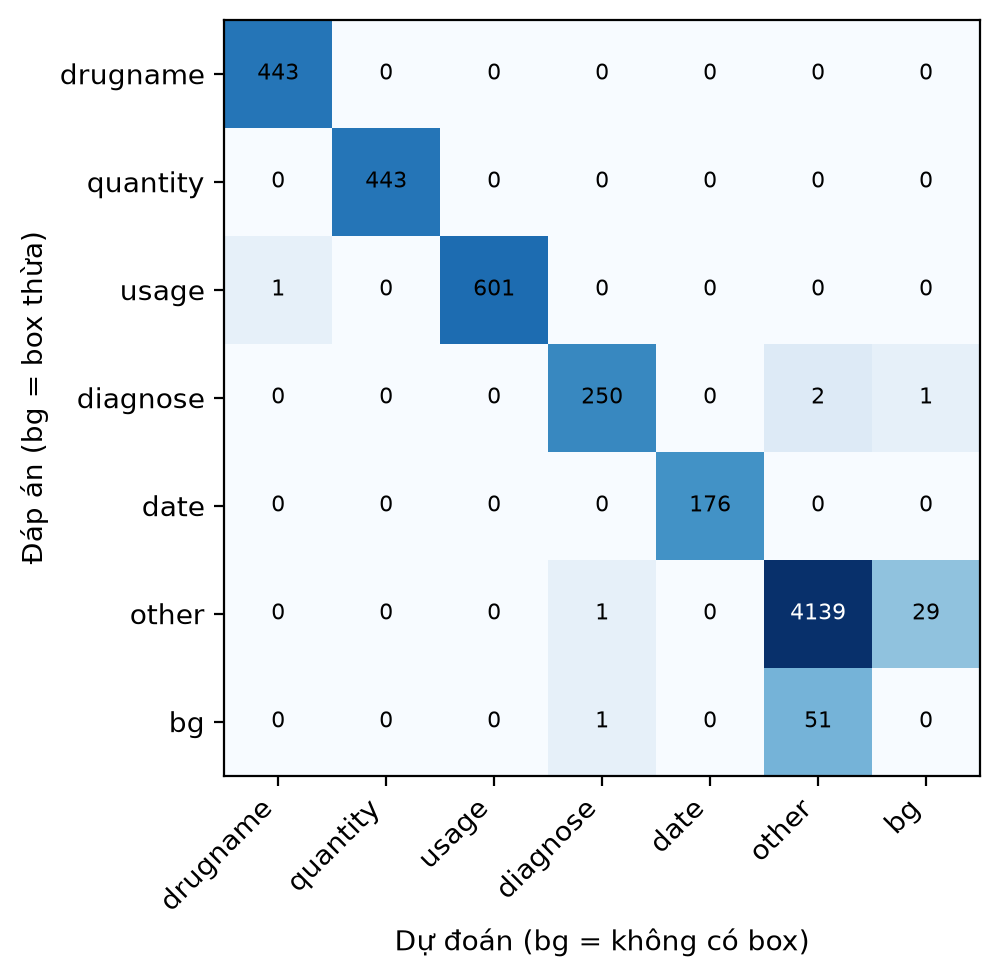
\includegraphics[width=0.42\linewidth]{e_b_detection/b2_confusion.png}
\caption{Ma trận nhầm lẫn của YOLOv8s. Hàng \texttt{bg} là khung thừa, cột \texttt{bg} là vùng bị bỏ sót.}\label{fig:confusion}
\end{figure}
\subsection{Nhận dạng chữ}\label{sec:e-recognize}
% ===== Mục 4.3 — Kết quả khối C (≈ 0,5 trang) =====
% Viết gì: bảng E-C1 trên vùng cắt theo KHUNG CHUẨN của test (cô lập khối C), nhận xét, 1 ca lỗi. Người: Khang.
% Nguồn số: C2/C3 toàn tập = lần chạy Kaggle (notebooks/finetune_vietocr.ipynb, ô kiểm tra cuối: C2 (0.0864, 0.1097, 0.8156),
% C3 (0.0329, 0.0437, 0.9229) = (CER, WER, khớp nguyên chuỗi)). Cột theo lớp + thời gian: chạy lại cục bộ.
VietOCR được tinh chỉnh bằng \path{code/notebooks/finetune_vietocr.ipynb} trên Kaggle T4 với \num{20000} vòng, batch 32, tốc độ học cực đại $3\cdot10^{-4}$ theo lịch one-cycle, tăng cường ảnh có sẵn của VietOCR và seed 42.
Dữ liệu là các vùng chữ có nhãn hợp lệ của tập huấn luyện (bỏ vùng rỗng, khung suy biến hoặc có ký tự ngoài bảng chữ của VietOCR), được cắt bằng \path{code/tools/to_vietocr.py} giống lúc suy luận, đệm 2~px và không phóng to.
Trọng số được chọn theo độ chính xác khớp nguyên chuỗi trên tập kiểm định.
Tham số \texttt{image\_max\_width} được nâng từ 512 lên 1024 vì với 512 khoảng 5\% vùng dài bị co chữ.
Hai bộ nhận dạng được bọc trong \path{code/src/recognize/vietocr_engine.py} và \path{code/src/recognize/tesseract_engine.py}.
Tesseract chạy với \texttt{--psm 7}, tức chế độ một dòng chữ.

Để tách riêng bước nhận dạng, mọi phương án đọc cùng 6086 vùng cắt theo khung chuẩn của tập kiểm tra, và kết quả thí nghiệm E-C1 được trình bày ở Bảng~\ref{tab:EC1}.

\begin{table}[H]
\centering
\caption{Nhận dạng chữ trên vùng cắt theo khung chuẩn, 176 ảnh kiểm tra trong E-C1. Khớp: tỉ lệ vùng đọc đúng nguyên chuỗi.}\label{tab:EC1}
\small
\begin{tabular}{lcccccc}
\toprule
\textbf{Phương án} & \textbf{CER} & \textbf{WER} & \textbf{Khớp} & \textbf{CER \texttt{drugname}} & \textbf{CER \texttt{quantity}} & \textbf{ms/vùng} \\
\midrule
Tesseract xám & \num{0.0689} & \num{0.1961} & \num{0.636} & \num{0.0363} & \num{0.0016} & \num{35.7} \\
Tesseract nhị phân & \num{0.0684} & \num{0.2002} & \num{0.619} & \num{0.0340} & \num{0.0168} & \num{37.8} \\
VietOCR gốc & \num{0.0864} & \num{0.1097} & \num{0.816} & \num{0.0275} & \num{0.0014} & \textbf{\num{17.3}} \\
VietOCR tinh chỉnh & \textbf{\num{0.0329}} & \textbf{\num{0.0437}} & \textbf{\num{0.923}} & \textbf{\num{0.0003}} & \textbf{\num{0.0004}} & \num{18.9} \\
\bottomrule
\end{tabular}
\par\smallskip{\footnotesize Nguồn: \path{result/e_c1_ocr/}. Tesseract chạy 8 luồng CPU, VietOCR chạy trên GPU RTX 3050 nên thời gian không so trực tiếp được.}
\end{table}

Tinh chỉnh giảm CER từ \num{0.0864} xuống \num{0.0329}, tức khoảng 62\%, và tăng tỉ lệ vùng đọc đúng nguyên chuỗi từ \num{0.816} lên \num{0.923}.
Mức giảm đến chủ yếu từ dòng chẩn đoán với CER từ \num{0.2325} xuống \num{0.0625} và dòng cách dùng từ \num{0.0123} xuống \num{0.0038}, còn tên thuốc và số lượng gần như không còn lỗi.
Tesseract có CER tổng thấp hơn VietOCR gốc vì đọc dòng chẩn đoán tốt hơn ở mức \num{0.0811} so với \num{0.2325}, nhưng đọc cách dùng kém hơn nhiều với \num{0.1039} so với \num{0.0123} nên WER và tỉ lệ đọc đúng nguyên chuỗi đều thua VietOCR gốc.
Nhị phân hóa Sauvola ở Tesseract nhị phân không đổi CER tổng và làm CER của số lượng tăng từ \num{0.0016} lên \num{0.0168}, nên không giúp ích.
Lỗi còn lại của VietOCR tinh chỉnh tập trung ở dòng chẩn đoán, trong đó có cả lỗi do nhãn sai ở Hình~\ref{fig:c3err}, Phụ lục~\ref{app:examples}.

\subsection{So sánh đầu-cuối}\label{sec:e-endtoend}
% Mục 4.4. So sánh đầu-cuối, bảng chính (khoảng 0,7 trang). Người viết: Thắng.
% Nguồn số: results/E-D1, results/E-D2/table.csv (code/experiments/e_d1.py, e_d2.py).
Khi chạy khối D trên khung và chữ chuẩn của tập kiểm tra (E-D1), F1 khoản thuốc đạt \num{1.000}.
Kết quả này chỉ cho thấy luật ghép nhất quán khi đầu vào đúng, chưa phải đánh giá độc lập, vì đáp án khoản thuốc cũng được dẫn xuất từ chính luật đó.
Kết quả chính của đồ án (E-D2) nằm ở Bảng~\ref{tab:ED2}.

\begin{table}[H]
\centering
\caption{Kết quả đầu-cuối trên 176 ảnh kiểm tra (E-D2). F1 khoản đòi hỏi tên đúng (CER $\le0{,}1$) và số lượng đúng; ngoặc vuông là khoảng tin cậy 95\% theo bootstrap.}\label{tab:ED2}
\footnotesize
\begin{tabularx}{\linewidth}{@{}Lcccccc@{}}
\toprule
\textbf{Pipeline} & \textbf{F1 khoản [CI 95\%]} & \textbf{Bỏ từ điển} & \textbf{F1 tên} & \textbf{SL đúng} & \textbf{Đơn đúng} & \textbf{s/ảnh} \\
\midrule
Chữ chuẩn (khung YOLO, chữ chuẩn)           & \num{1.0000} & \num{1.0000} & \num{1.0000} & \num{1.0000} & \num{1.0000} & --- \\
\midrule
(i) Cổ điển (B cổ điển, Tesseract, D)       & \num{0.9487} [\num{0.9316}; \num{0.9647}] & \num{0.9161} & \num{0.9580} & \num{0.9187} & \num{0.8011} & \textbf{\num{1.16}} \\
(ii) Lai (YOLO, Tesseract, D)              & \num{0.9865} [\num{0.9736}; \num{0.9977}] & \num{0.9549} & \num{0.9955} & \num{0.9865} & \num{0.9716} & \num{1.38} \\
(iv) YOLO, VietOCR công bố (C2), D          & \textbf{\num{0.9966}} [\num{0.9895}; \num{1.0000}] & \num{0.9514} & \textbf{\num{0.9966}} & \num{0.9955} & \textbf{\num{0.9943}} & \num{3.77} \\
(iii) YOLO, VietOCR tinh chỉnh (C3), D      & \textbf{\num{0.9966}} [\num{0.9930}; \num{1.0000}] & \textbf{\num{0.9966}} & \textbf{\num{0.9966}} & \textbf{\num{1.0000}} & \num{0.9830} & \num{3.37} \\
(v) VLM zero-shot (Qwen3.8-27B)              & \textbf{\num{0.9966}} [\num{0.9892}; \num{1.0000}] & \num{0.9875} & \textbf{\num{0.9966}} & \num{0.9932} & \textbf{\num{0.9943}} & --- \\
\bottomrule
\end{tabularx}
\par\smallskip{\footnotesize Nguồn: \path{result/e_d2_endtoend/}, \path{result/runtime/}. Cột ``Bỏ từ điển'' là F1 khoản khi tắt bước D4; cột ``s/ảnh'' là thời gian khối B+C (VLM gọi qua API từ xa, có 1/176 ảnh lỗi định dạng JSON).}
\end{table}

Pipeline chính (iii) đạt F1 khoản thuốc \num{0.9966} (CI 95\%: $[\num{0.9930}; \num{1.0000}]$), đúng 100\% số lượng (\num{1.0000}) và ngày kê đơn (\num{1.0000}), chỉ kém \num{0.0034} điểm so với mức trần dùng chữ chuẩn (\num{1.0000}).
Từ điển tên thuốc (D4) giúp tăng mạnh F1 khoản khi OCR còn lỗi ký tự: VietOCR công bố (iv) tăng \num{0.0452} điểm (từ \num{0.9514} lên \num{0.9966}), bản lai (ii) tăng \num{0.0316} điểm (\num{0.9549} lên \num{0.9865}), bản cổ điển (i) tăng \num{0.0326} điểm (\num{0.9161} lên \num{0.9487}) và VLM (v) tăng \num{0.0091} điểm (\num{0.9875} lên \num{0.9966}), trong khi VietOCR tinh chỉnh (iii) giữ nguyên \num{0.9966} cả khi bỏ từ điển nhờ CER tên thuốc chỉ còn \num{0.0003}.
So với VLM zero-shot Qwen3.8-27B (v), pipeline chính (iii) đạt cùng F1 khoản \num{0.9966} khi có từ điển nhưng cao hơn khi bỏ từ điển (\num{0.9966} so với \num{0.9875}), đạt độ chính xác tuyệt đối ở cả số lượng và ngày kê đơn (\num{1.0000} so với \num{0.9932} và \num{0.9943}), và không bị lỗi cú pháp đầu ra (VLM có 1/176 ảnh trả về JSON hỏng định dạng).

\subsection{Phân tích lỗi và độ bền}\label{sec:e-ablation}
% Mục 4.4.4. Nguồn lỗi còn lại (E-X1). Người viết: Hiếu. Nguồn số: results/E-X1/table.csv.
Nhóm thay lần lượt bước phát hiện và bước nhận dạng bằng nhãn chuẩn Ground Truth để tách nguồn lỗi, thí nghiệm E-X1, ở Bảng~\ref{tab:EX1}.

\begin{table}[H]
\centering
\caption{Kết quả khi thay từng bước bằng nhãn chuẩn Ground Truth (E-X1).}\label{tab:EX1}
\footnotesize
\begin{tabular}{llcccc}
\toprule
\textbf{Phát hiện} & \textbf{Nhận dạng} & \textbf{F1 khoản} & \textbf{F1 tên} & \textbf{SL đúng} & \textbf{Đơn đúng} \\
\midrule
Ground Truth & Ground Truth & \num{1.0000} & \num{1.0000} & \num{1.0000} & \num{1.0000} \\
Ground Truth & VietOCR tinh chỉnh & \num{1.0000} & \num{1.0000} & \num{1.0000} & \num{1.0000} \\
YOLOv8s & Ground Truth & \num{1.0000} & \num{1.0000} & \num{1.0000} & \num{1.0000} \\
YOLOv8s & VietOCR tinh chỉnh & \num{0.9966} & \num{0.9966} & \num{1.0000} & \num{0.9830} \\
\bottomrule
\end{tabular}
\end{table}

Khi dùng khung chuẩn với chữ do VietOCR tinh chỉnh đọc, hoặc khung YOLOv8s với chữ chuẩn, F1 khoản đều đạt \num{1.0000}.
Mức giảm \num{0.0034} điểm ở pipeline chính, ứng với 173/176 đơn đúng hoàn toàn, chỉ xuất hiện khi ghép đồng thời khung dự đoán của YOLOv8s với chữ của VietOCR tinh chỉnh.

\subsection{Thời gian chạy}\label{sec:e-runtime}
% ===== Mục 4.6 — Thời gian chạy (≈ 0,25 trang) =====
% Viết gì: giây/ảnh từng khối, trung bình 176 ảnh test. Người: Hiếu.
Bảng~\ref{tab:runtime} cho thời gian trung bình mỗi ảnh trên máy cá nhân với CPU Core i7-12700H và GPU RTX~3050.

\begin{table}[H]
\centering
\caption{Thời gian trung bình mỗi ảnh tính bằng giây. Khối A đo trên 50 ảnh L0 bằng CPU, khối B và C đo trên 176 ảnh kiểm tra bằng GPU, khối D lấy theo khoảng đo được.}\label{tab:runtime}
\small
\begin{tabular}{ccccc}
\toprule
\textbf{A} & \textbf{B} & \textbf{C} & \textbf{D} & \textbf{Tổng} \\
\midrule
\num{0.12} & \num{0.05} & \num{3.32} & $\approx\num{0.02}$ & $\approx\num{3.5}$ \\
\bottomrule
\end{tabular}
\par\smallskip{\footnotesize Nguồn: \path{result/e_a3_runtime/}, \path{result/runtime/}.}
\end{table}

Khối C chiếm gần hết thời gian vì VietOCR đọc mọi vùng, kể cả khoảng 68\% số vùng thuộc lớp \texttt{other} mà khối D không dùng.
Bỏ qua các vùng này sẽ giảm đáng kể thời gian của khối C.


\section{Thảo luận}\label{sec:discussion}
% ===== Mục 5 — Thảo luận (≈ 0,75 trang) =====
% Viết gì: mỗi ý 2–3 câu CÓ SỐ từ mục 4. Người: Hiếu + Thắng.
\subsection{Khi nào cổ điển đủ, khi nào cần học sâu}
\TODO{So dòng (i)/(ii) với (iii) ở Bảng~\ref{tab:ED2} và E-B1: cổ điển tìm vùng chữ được nhưng không phân lớp, nên phải dựa vào luật trên chữ OCR — lỗi OCR kéo theo lỗi phân lớp. Phần nào cổ điển vẫn đáng dùng (tiền xử lý khi ảnh xấu, theo E-A1)}

\subsection{Học sâu theo khối so với VLM đầu-cuối}
\TODO{Thắng: VLM mạnh ở đâu (không cần huấn luyện, đọc ngữ cảnh), yếu ở đâu (bịa tên/liều, chậm, phụ thuộc API, gửi ảnh y tế ra ngoài). Dẫn số từ Bảng~\ref{tab:ED2}}

\subsection{Hạn chế}
\begin{itemize}
  \item VAIPE là ảnh in máy, sạch, cùng một mẫu đơn; kết quả chưa được kiểm chứng trên ảnh chụp điện thoại thật hay mẫu đơn của bệnh viện khác. Bộ suy giảm tổng hợp (Mục~\ref{sec:items-gt}) chỉ mô phỏng một phần.
  \item Đáp án khoản thuốc được dẫn xuất bằng chính luật của \khoi{D}, chỉ soát bằng mắt \KQ{số ảnh} ảnh; E-D1 $=1{,}000$ vì thế chỉ chứng tỏ luật nhất quán, không chứng tỏ đáp án đúng tuyệt đối.
  \item Từ điển tên thuốc lấy từ tập huấn luyện; \KQ{\% OOV} tên thuốc kiểm tra nằm ngoài từ điển và không được hưởng lợi.
  \item \TODO{phần đã cắt vì thời gian: E-B3 (đường cong dữ liệu), E-C2 (tiền xử lý vùng cắt), E-D3; Tesseract / B cổ điển nếu không chạy}
\end{itemize}

\subsection{Hướng phát triển}
\TODO{1--2 câu: thu ảnh chụp thật để đánh giá; huấn luyện YOLO/VietOCR có tăng cường suy giảm; bỏ vùng \texttt{other} trước OCR để tăng tốc; từ điển thuốc quốc gia thay cho từ điển tập huấn luyện}


\section{Kết luận}\label{sec:conclusion}
% ===== Mục 5.1 — Kết luận (≈ 4–5 câu) =====
% Người: Hiếu.
Đồ án xây dựng pipeline trích xuất đơn thuốc gồm tiền xử lý cổ điển, YOLOv8s, VietOCR tinh chỉnh và luật ghép khoản có từ điển.
Trên 176 ảnh kiểm tra VAIPE, pipeline đạt F1 khoản thuốc \KQ{F1 [CI]}, so với \KQ{F1 VLM} của VLM zero-shot và \KQ{F1 cổ điển} của pipeline cổ điển.
Tinh chỉnh VietOCR giảm CER từ \num{0.0864} xuống \num{0.0329}.
\TODO{1 câu về vai trò tiền xử lý cổ điển theo E-A1}
\TODO{1 câu về hạn chế chính: chưa kiểm chứng trên ảnh chụp thật}


\section{Phân công}\label{sec:contrib}
% ===== Mục 6 — Phân công =====
% Người: Hiếu. Kiểm lại với cả nhóm trước khi nộp.
Mỗi thành viên phụ trách một khối của pipeline và đóng góp 25\% khối lượng công việc (Bảng~\ref{tab:contrib}).

\begin{table}[H]
\centering
\caption{Phân công công việc.}\label{tab:contrib}
\small
\begin{tabularx}{\linewidth}{lX}
\toprule
\textbf{Thành viên} & \textbf{Phần việc} \\
\midrule
Trần Trung Hiếu (nhóm trưởng) & \Khoi{A} tiền xử lý; bộ ảnh suy giảm; E-A1, E-X1; tích hợp pipeline, demo; ghép báo cáo, slide, đóng gói và nộp \\
Nguyễn Anh Trường & \Khoi{B}: chuyển nhãn YOLO, huấn luyện YOLOv8s trên Kaggle, chọn ngưỡng; E-B1, E-B2 \\
Đào Văn Khang & \Khoi{C}: sinh dữ liệu vùng cắt, tinh chỉnh VietOCR trên Kaggle, engine nhận dạng; E-C1; tệp bàn giao B+C cho đầu-cuối \\
Nguyễn Tiến Thắng & \Khoi{D}: luật ghép khoản, chuẩn hóa, từ điển, đối chứng VLM; đáp án khoản thuốc; E-D1, E-D2 \\
\bottomrule
\end{tabularx}
\end{table}


\section{Khai báo sử dụng AI}\label{sec:ai}
% Mục 8. Khai báo sử dụng AI. Mỗi người điền 1 đến 2 câu. Người viết: Hiếu tổng hợp.
Nhóm có dùng Claude (Anthropic) qua Claude Code\TODO{, và công cụ khác nếu có} để viết khung mã nguồn các khối, script chuyển nhãn, notebook huấn luyện và script thí nghiệm, viết kiểm thử đơn vị, sửa lỗi, và soạn bản nháp cũng như định dạng báo cáo, slide.

Nhóm tự chọn đề tài, chốt phương pháp và tham số, chạy huấn luyện trên Kaggle, chạy và đọc kết quả thí nghiệm, soát đáp án bằng mắt và chỉnh lại toàn bộ báo cáo.
Phần việc cụ thể của từng người như sau.
\begin{itemize}
  \item Hiếu: \TODO{1 đến 2 câu}
  \item Trường: \TODO{1 đến 2 câu}
  \item Khang: \TODO{1 đến 2 câu, ví dụ AI viết notebook tinh chỉnh và engine VietOCR, còn Khang chạy huấn luyện, chọn \texttt{image\_max\_width} 1024 sau khi thấy vùng dài bị co và đối chiếu kết quả}
  \item Thắng: \TODO{1 đến 2 câu}
\end{itemize}

Về cách kiểm tra, mọi module có kiểm thử đơn vị (\texttt{pytest}, \KQ{số} bài).
Mọi con số trong báo cáo lấy từ tệp kết quả do script trong \path{code/experiments/} hoặc notebook sinh ra và chạy lại được với seed 42.
Tham số được chọn trên tập kiểm định, còn tập kiểm tra chỉ chạy một lần.


% ===================== PHỤ LỤC =====================
\clearpage
\appendix
\section{Bảng tham số đầy đủ}\label{app:params}
% ===== Phụ lục A — Bảng tham số đầy đủ =====
% Viết gì: mọi tham số, giá trị chọn, khoảng đã thử (nếu có), lý do. Mỗi người điền dòng của khối mình.
\begin{table}[H]
\centering
\caption{Tham số của pipeline. Dấu ``---'' nghĩa là không dò, dùng giá trị mặc định hoặc theo lý do ghi bên cạnh.}\label{tab:params}
\footnotesize
\begin{tabularx}{\linewidth}{@{}l >{\raggedright\arraybackslash}p{3.7cm} >{\raggedright\arraybackslash}p{2.6cm} >{\raggedright\arraybackslash}p{2.2cm} L@{}}
\toprule
\textbf{Khối} & \textbf{Tham số} & \textbf{Giá trị} & \textbf{Đã thử} & \textbf{Lý do} \\
\midrule
A1 & Ngưỡng Canny & 50 / 150 & --- & \TODO{} \\
A1 & Diện tích tứ giác tối thiểu & 20\% ảnh & --- & Loại tứ giác nhỏ (bảng, ô) \\
A2 & Khoảng góc, bước & $\pm10^\circ$, $0{,}25^\circ$ & --- & Nghiêng chụp tay thường $<10^\circ$ \\
A2 & Sauvola cửa sổ, $k$ & 31, 0,2 & --- & \TODO{} \\
A3 & Phần tử cấu trúc phép đóng & $81\times81$ & \KQ{} & Lớn hơn nhiều lần chiều cao chữ \\
A4 & Lọc trung vị & $3\times3$ & --- & \TODO{} \\
A5 & CLAHE giới hạn cắt, lưới & 2,0; $8\times8$ & --- & \TODO{} \\
\midrule
B & Mô hình, kích thước ảnh & YOLOv8s, 1024 & --- & Chữ cao 15--25~px \\
B & Epoch, batch, dừng sớm & 50, 16, 15 & --- & Vừa thời gian Kaggle \\
B & \texttt{fliplr}, mosaic & 0; 0,5 & --- & Lật ngang làm hỏng chữ \\
B & Ngưỡng tin cậy & 0,443 & quét trên tập kiểm định & F1 trung bình 6 lớp lớn nhất \\
B & Ngưỡng NMS & 0,7 & --- & Mặc định Ultralytics \\
\midrule
C & Kiến trúc & \texttt{vgg\_transformer} & --- & Trọng số tiếng Việt có sẵn \\
C & Số vòng, batch, lr & \num{20000}, 32, $3\cdot10^{-4}$ & --- & Vừa thời gian Kaggle T4 \\
C & Chiều rộng ảnh tối đa & 1024~px & 512 & 512 làm co $\approx5\%$ vùng dài \\
C & Đệm vùng cắt & 2~px & --- & Giữ dấu, nét sát khung \\
C & Giải mã & tham lam & --- & Nhanh; \TODO{beam search có giúp không} \\
\midrule
D & Ngưỡng tin cậy hỏi lại bằng luật & 0,5 & --- & \TODO{} \\
D & IoU trùng & 0,7 & --- & \TODO{} \\
D & Từ điển $\tau_{\text{cao}}$, $\tau_{\text{thấp}}$, lề & 90, 80, 5 & trên tập kiểm định & Chặn kéo sai liều; xem Mục~\ref{sec:m-assemble} \\
D & Khớp tên khi chấm & CER $\le0{,}1$ & --- & Cho phép lỗi nhỏ không đổi nghĩa \\
\bottomrule
\end{tabularx}
\end{table}

\section{Ví dụ kết quả và ca lỗi}\label{app:examples}
% ===== Phụ lục — Ví dụ kết quả và ca lỗi =====
% Hai nhóm hình: (1) kết quả và ca lỗi của pipeline, (2) minh họa tiền xử lý. Chú thích hình tự đủ nghĩa, không lặp câu dẫn.
\subsection*{Kết quả của pipeline}
Hình~\ref{fig:example} là đầu ra đầu-cuối trên một đơn thuốc, Hình~\ref{fig:confusion} là ma trận nhầm lẫn của YOLOv8s, và Hình~\ref{fig:c3err} là các ca VietOCR tinh chỉnh đọc khác nhãn.

\begin{figure}[H]
\centering
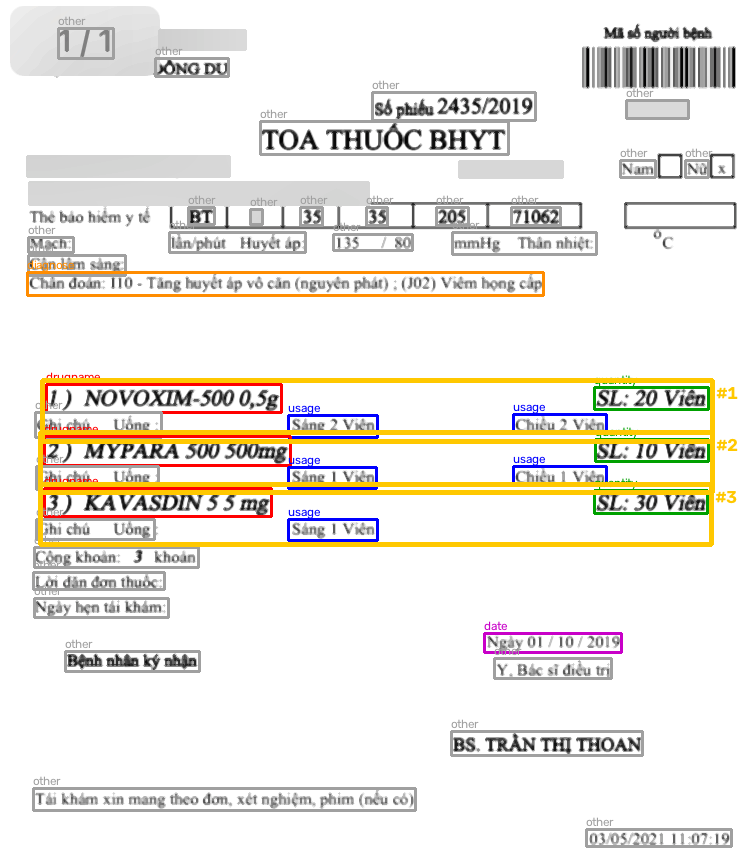
\includegraphics[width=0.5\linewidth]{common/pipeline_example.png}
\caption{Kết quả đầu-cuối trên một ảnh mẫu VAIPE sau tiền xử lý. Khung màu theo lớp YOLO gồm đỏ (\texttt{drugname}), xanh lá (\texttt{quantity}), xanh dương (\texttt{usage}), cam (\texttt{diagnose}), tím (\texttt{date}) và xám (\texttt{other}). Khung vàng \#1 đến \#3 là ba khoản thuốc sau bước ghép khoản. Cả ba khoản đúng tên, số lượng và cách dùng, lỗi duy nhất là mã bệnh ``I10'' bị đọc thành ``110'', cùng kiểu lỗi với Hình~\ref{fig:c3err}(c).}\label{fig:example}
\end{figure}

\begin{figure}[H]
\centering
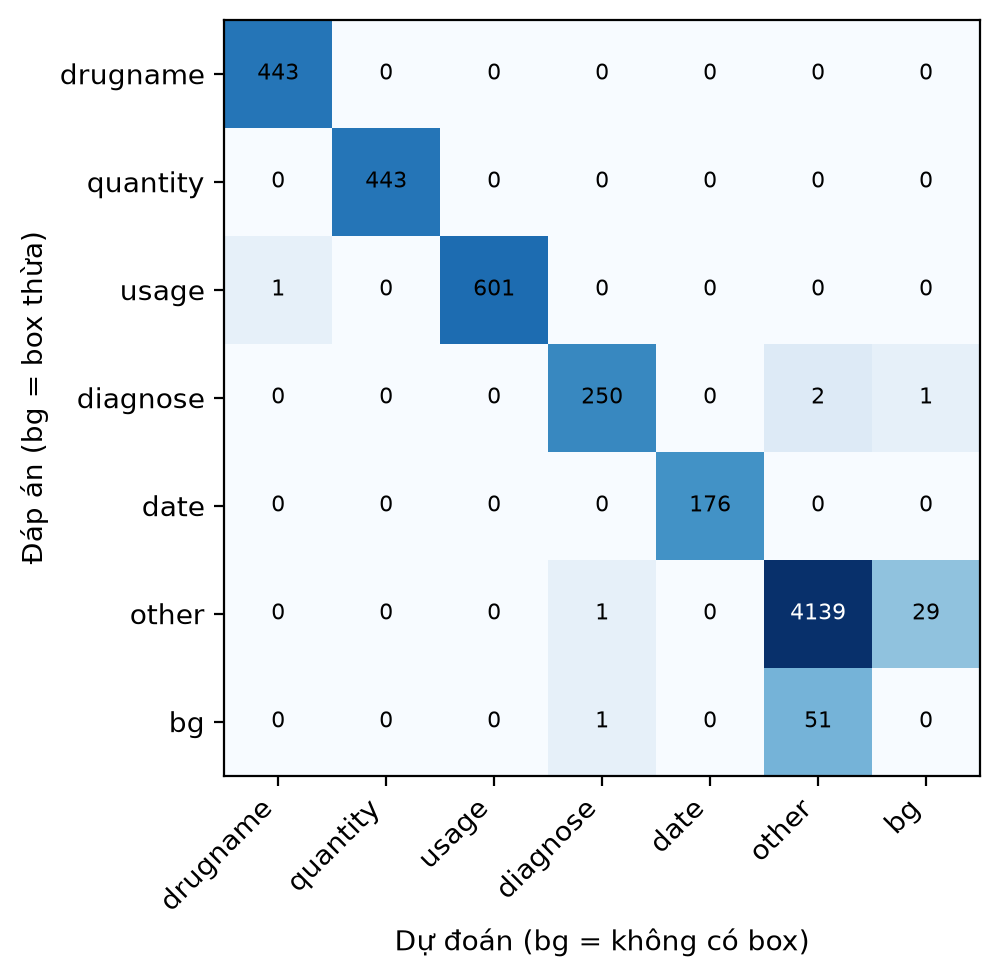
\includegraphics[width=0.42\linewidth]{e_b_detection/b2_confusion.png}
\caption{Ma trận nhầm lẫn của YOLOv8s trên 176 ảnh kiểm tra với IoU $\ge0{,}5$. Hàng \texttt{bg} là khung dự đoán thừa, cột \texttt{bg} là vùng chuẩn bị bỏ sót. Lỗi chủ yếu là sót hoặc thừa khung \texttt{other}; rất ít vùng bị nhầm giữa các lớp.}\label{fig:confusion}
\end{figure}

\begin{figure}[H]
\centering
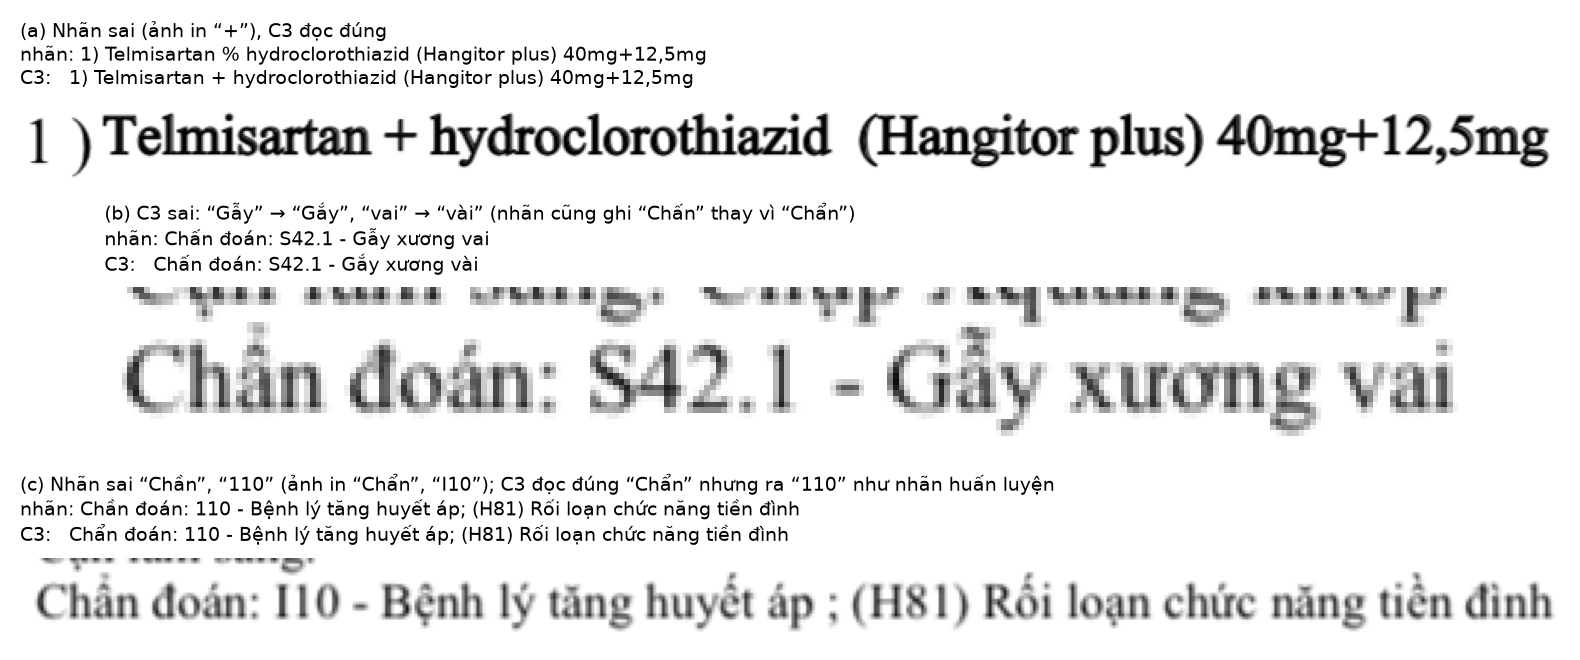
\includegraphics[width=0.9\linewidth]{e_c1_ocr/c3_errors.png}
\caption{Ba vùng VietOCR tinh chỉnh đọc khác nhãn. (a) Nhãn sai, mô hình đọc đúng. (b) Mô hình sai dấu từ ``Gẫy'' thành ``Gắy'' và từ ``vai'' thành ``vài''. (c) Nhãn huấn luyện ghi ``110'' thay vì ``I10'' và mô hình đọc theo nhãn.}\label{fig:c3err}
\end{figure}

\subsection*{Minh họa tiền xử lý}
Hình~\ref{fig:levels} là ba mức suy giảm dùng trong thí nghiệm độ bền, Hình~\ref{fig:shadow} minh họa bước khử bóng, và Hình~\ref{fig:asteps} là một ảnh suy giảm nặng qua đủ năm bước tiền xử lý.

\begin{figure}[H]
\centering
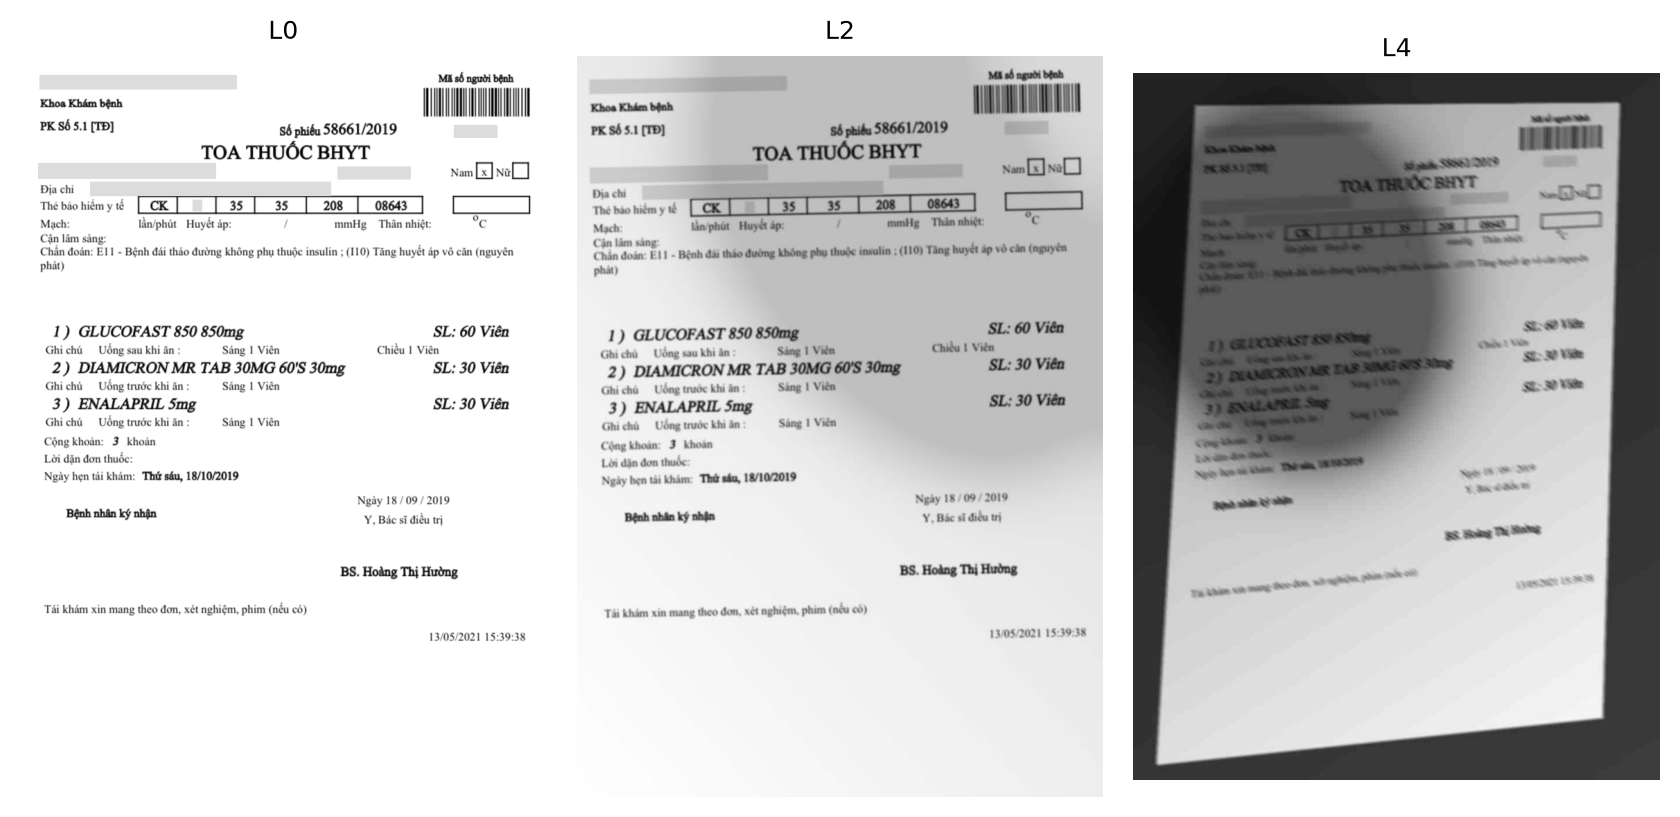
\includegraphics[width=0.95\linewidth]{fig_enhance/a_levels.png}
\caption{Một ảnh kiểm tra ở ba mức suy giảm là ảnh gốc, suy giảm nhẹ và suy giảm nặng.}\label{fig:levels}
\end{figure}

\begin{figure}[H]
\centering
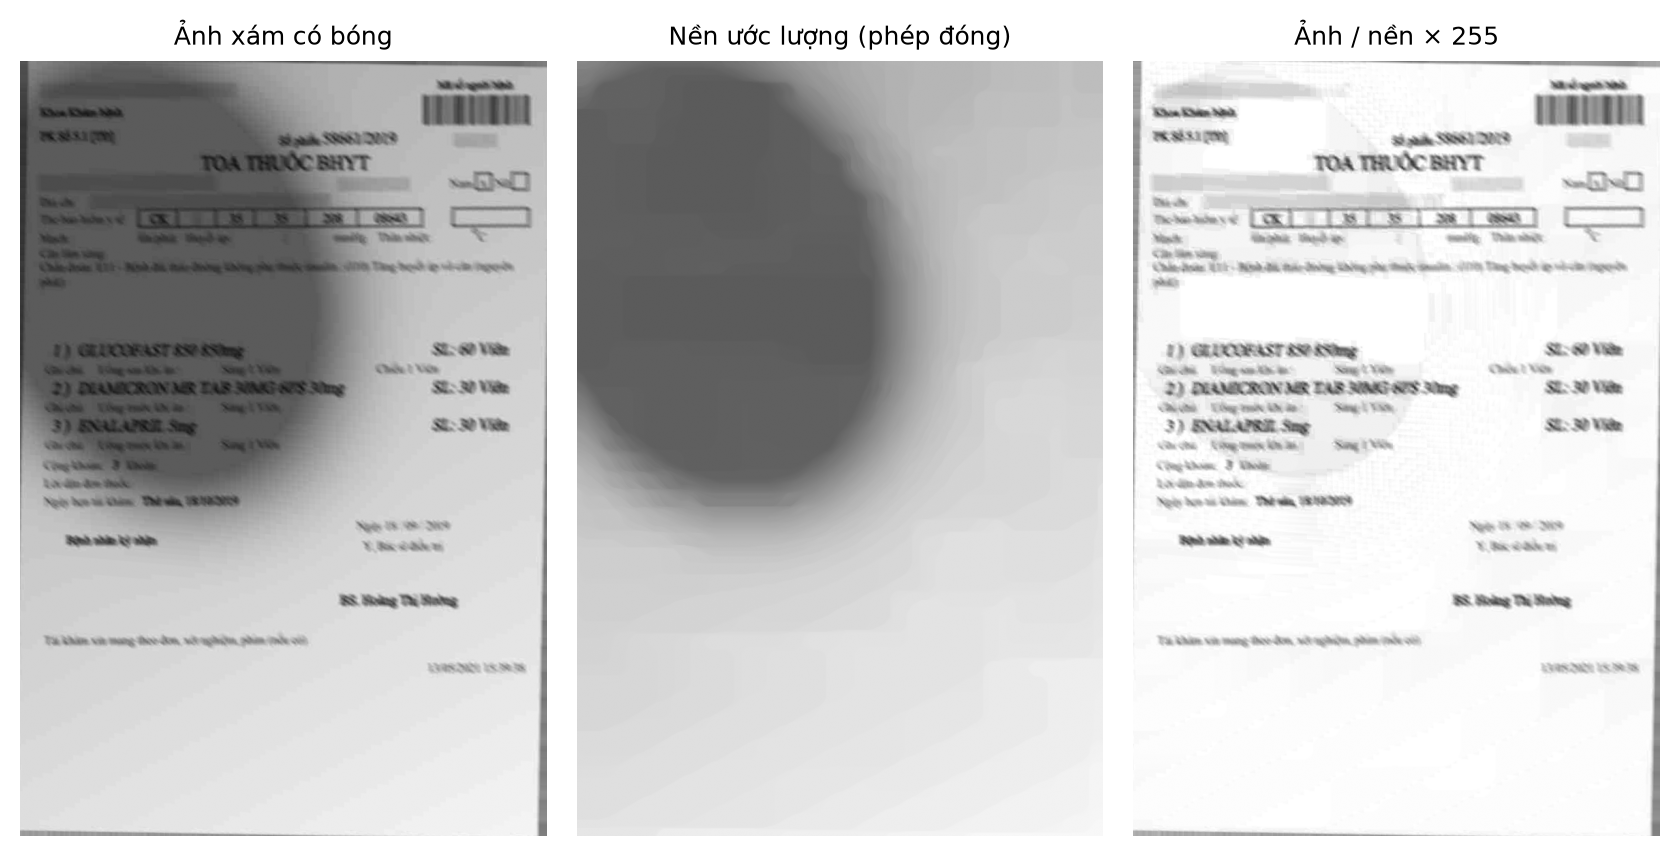
\includegraphics[width=0.95\linewidth]{fig_enhance/a_shadow.png}
\caption{Khử bóng: ảnh xám có bóng, nền ước lượng bằng phép đóng $81\times81$, ảnh sau khi chia cho nền.}\label{fig:shadow}
\end{figure}

\begin{figure}[H]
\centering
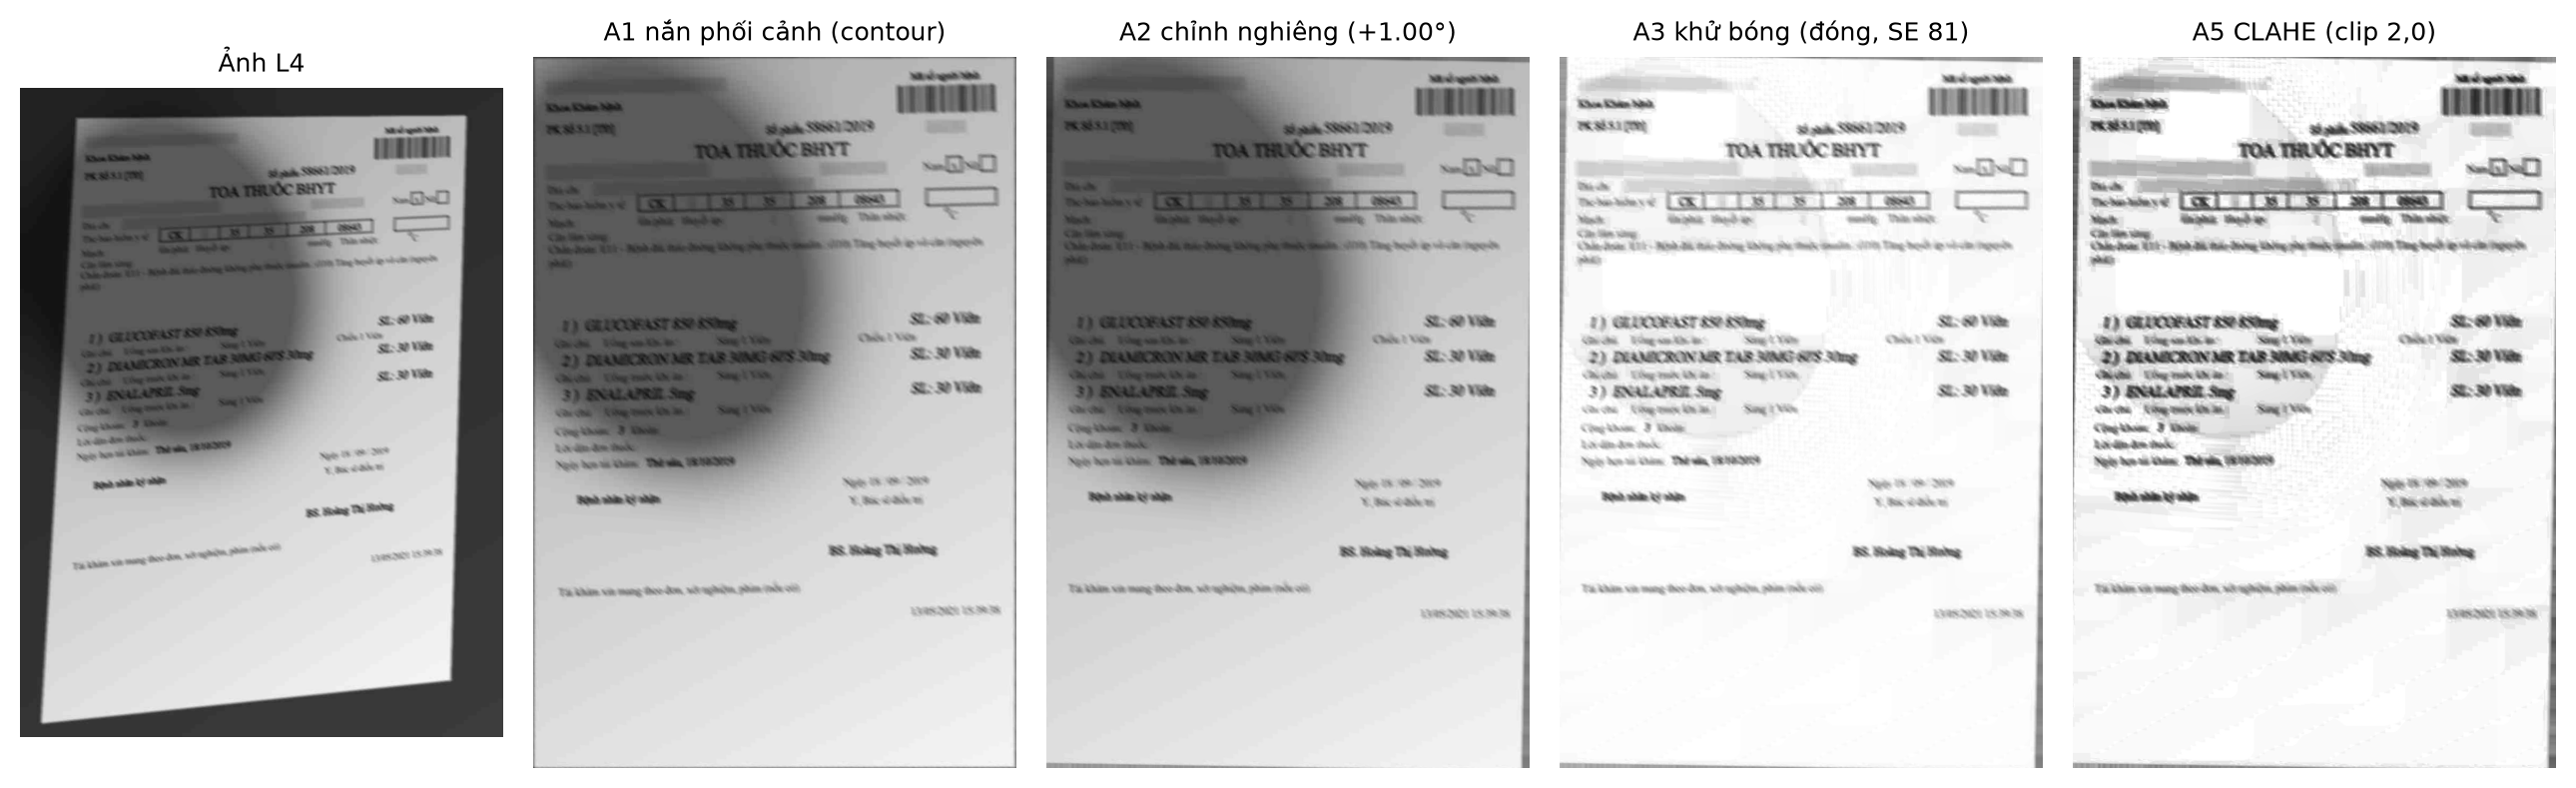
\includegraphics[width=\linewidth]{fig_enhance/a_steps.png}
\caption{Ảnh suy giảm nặng qua các bước tiền xử lý. Nắn phối cảnh và chia nền loại bỏ nền bàn tối và vùng bóng, nhưng độ mờ vẫn còn và CLAHE làm xuất hiện vài vệt khối ở vùng nền.}\label{fig:asteps}
\end{figure}


% Danh mục tài liệu tham khảo đặt cuối bài, bắt đầu ở trang mới
\clearpage
\phantomsection
\printbibliography[heading=bibintoc,title={Tài liệu tham khảo}]

\end{document}
